\documentclass[12pt]{article}
\usepackage{setspace}  % To use linespacing
\usepackage{indentfirst} % Indents first line after sections
\usepackage{amssymb} % For \mathbb
\usepackage{enumerate} % For changing labels of enumerate
\usepackage[margin=1in]{geometry} % For editing margins
\usepackage{tikz} % Tikz drawing for graphs
\usetikzlibrary{arrows.meta} % Allows customizing arrows
\usetikzlibrary{backgrounds} % For framing a tikzpicture
\usetikzlibrary{calc, through}
\usetikzlibrary{decorations.markings}
\usetikzlibrary{arrows}
\usetikzlibrary{positioning}
\usepackage{amsmath}

% Make new commands
\newcommand{\N}{\mathbb{N}}
\newcommand{\R}{\mathbb{R}}
\newcommand{\Z}{\mathbb{Z}}
\newcommand{\abs}[1]{\left|#1\right|}
\newcommand{\paren}[1]{\left(#1\right)}
\newcommand{\fivespace}{\space\space\space\space\space}

\newcommand{\be}{\begin{enumerate}}
\newcommand{\ee}{\end{enumerate}}
\newcommand{\seti}[1]{\setcounter{enumi}{#1}}
\newcommand{\setii}[1]{\setcounter{enumii}{#1}}

% Start main document
\begin{document}
\onehalfspacing
\hfill Frank Cline

\hfill Math 307

\hfill HW 9

% Figure 1 a
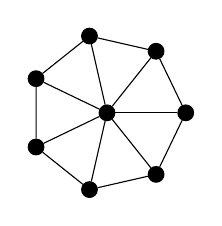
\begin{tikzpicture}
\foreach \i in {0, 1, ..., 6}{
\node[draw, circle, fill = black, inner sep = 2pt] (\i) at (360/7*\i:1){};}
\node[draw, circle, fill = black, inner sep = 2pt] (7) at (0,0){};
\foreach \i in {0, 1, ..., 6}{
\draw let \n1 = {int(mod(\i+1,7))} in (\i) -- (\n1);
\draw (\i) -- (7);}
\end{tikzpicture}

% Figure 1 b
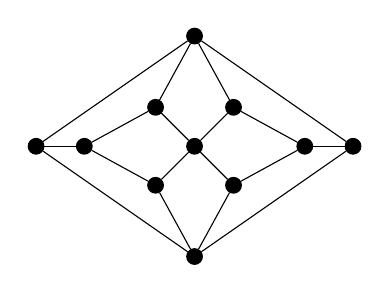
\begin{tikzpicture}[every node/.style={draw, circle, fill = black, 
inner sep = 2pt}]
\foreach \i in {0, 1, 2, 3}{
\node[] (\i) at (360/4*\i+45:.7){};}
\foreach \i in {4, 5, 6, 7}{
\node[] (\i) at (360/4*\i:1.4){};}
\node (8) at (0,0) {};
\node[ right = .4cm of 4]  (9) {};
\node [left = .4cm of 6] (10) {};
\foreach \i/\j in {8/0, 8/1, 8/2, 8/3, 0/5, 5/1, 1/6, 6/2, 2/7, 7/3, 3/4, 5/10, 10/7, 5/9, 9/7, 0/4, 6/10, 4/9}{
\draw (\i) -- (\j);}
\end{tikzpicture}

% Figure 1 c
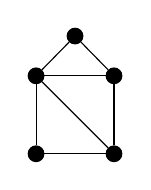
\begin{tikzpicture}[every node/.style={draw, circle, fill = black, 
inner sep = 2pt}]
\foreach \i in {0, 1, 2, 3}{
\node[] (\i) at (360/4*\i+45:.7){};}
\node[draw, circle, fill = black, inner sep = 2pt] (5) at (0,1){};
\foreach \i in {0, 1, ..., 3}{
\draw let \n1 = {int(mod(\i+1,4))} in (\i) -- (\n1);}
\draw (1) -- (5) (5) --(0) (1) -- (3);
\end{tikzpicture}

% Figure 1 d
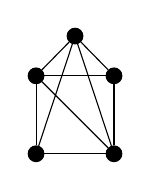
\begin{tikzpicture}[every node/.style={draw, circle, fill = black, 
inner sep = 2pt}]
\foreach \i in {0, 1, 2, 3}{
\node[] (\i) at (360/4*\i+45:.7){};}
\node[draw, circle, fill = black, inner sep = 2pt] (5) at (0,1){};
\foreach \i in {0, 1, ..., 3}{
\draw let \n1 = {int(mod(\i+1,4))} in (\i) -- (\n1);}
\draw (1) -- (5) (5) --(0) (5) -- (2) (5) -- (3) (1)--(3);
\end{tikzpicture}

% Figure 1 e
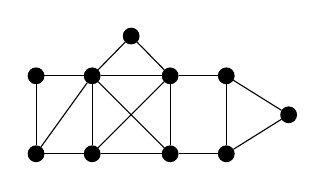
\begin{tikzpicture}[every node/.style={draw, circle, node distance = .5cm, fill = black, 
inner sep = 2pt}]
\foreach \i in {0, 1, 2, 3}{
\node[] (\i) at (360/4*\i+45:.7){};}
\node[] (5) at (0,1){};
\foreach \i in {0, 1, ..., 3}{
\draw let \n1 = {int(mod(\i+1,4))} in (\i) -- (\n1);}
\draw (1) -- (5) (5) --(0) ;
\node[left = of 2] (6){};
\node[left = of 1] (7){};
\node[right = of 0] (8){};
\node[right = of 3] (9){};
\node[] (10) at (2,0) {};
\foreach \i/\j in {1/7, 7/6, 6/2, 1/6, 0/8, 8/9, 9/3, 8/9, 9/10, 1/3, 0/2, 10/8}{
\draw (\i) -- (\j);}
\end{tikzpicture}

% Figure 2
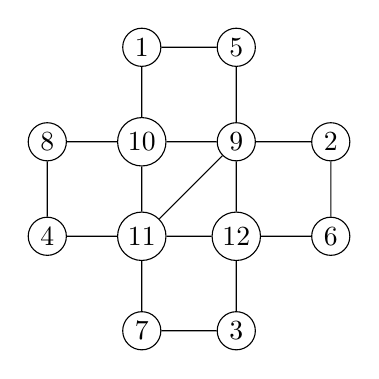
\begin{tikzpicture}[every node/.style={draw, circle, inner sep = 2 pt}, scale=1.2]
\node (1) at (0,2) {1};
\node  (2) at (2,1) {2};
\node  (3) at (1,-1) {3};
\node (4) at (-1,0) {4};
\node (5) at (1,2) {5};
\node (6) at (2,0) {6};
\node (7) at (0,-1) {7};
\node (8) at (-1,1) {8};
\node (9) at (1,1) {9};
\node (10) at (0,1) {10};
\node (11) at (0,0) {11};
\node (12) at (1,0) {12};
\draw (10) -- (1) -- (5) -- (9) -- (2) -- (6) -- (12) -- (3) -- (7) -- (11) -- (4) -- (8) -- (10) -- (9) -- (12) -- (11) -- (10) (11) --(9);
\end{tikzpicture}

% Command for Figure 3
\newcommand{\grotzsch}[1]{

\begin{tikzpicture}[every node/.style={draw, circle, fill = black, 
inner sep = 2pt}]
%
\pgfmathtruncatemacro{\result}{#1-1}
\pgfmathtruncatemacro{\endNum}{#1*2}
\pgfmathtruncatemacro{\resultNum}{#1*2-1}
\pgfmathsetmacro{\angle}{360/#1}
%
\foreach \i in {0, 1, ..., \result}{
\node[] (\i) at (\angle*\i:2){};
\path let \n1={int(\i+#1)} in node[]  (\n1) at  (\angle*\i:1){};
}
\node (\endNum) at (0,0){};
\foreach \i in {0, ..., \result}{
\draw let \n1 = {int(mod(\i+1,#1))} in (\i) -- (\n1);
}
\foreach \i in {#1, ..., \resultNum}{
\draw let \n1 = {int(mod(\i+1,#1))} in (\i) -- (\n1);
\draw let \n1 = {int(mod(\i-1,#1))} in (\i) -- (\n1);
\draw (\i) -- (\endNum);
}
\end{tikzpicture}
}

% Figure 3 a
\grotzsch{5}

% Figure 3 b
\grotzsch{6}


% PROBLEMS
\section*{Problems 1-7}

DO WORK HERE

\end{document}















